%%%%%%%%%%%%%%%%%%%%%%%%%%%%%%%%%%%%%%%%%%%%%%%%%%%%%%%%%%%%%%%%%%%%%%%%
% Plantilla TFG/TFM
% Universidad de A Coruña. Facultad de Informática
% Realizado por: Welton Vieira dos Santos
% Modificado: Welton Vieira dos Santos
% Contacto: welton.dossantos@udc.es
%%%%%%%%%%%%%%%%%%%%%%%%%%%%%%%%%%%%%%%%%%%%%%%%%%%%%%%%%%%%%%%%%%%%%%%%


\chapter{Modelo de conocimiento}
\newpage
\section{Fase de identificación}
\subsection{Tareas del formulario OM-3}
Las tareas elegidas para este modelo conceptual han sido las tareas 2, 3 y 4 del OM-3 (Tabla \ref{tab:IdentificacionOM3}), que corresponden con \textbf{Generar lista de entregas según ruta asignada}, \textbf{Determinar los recursos disponibles por la sucursal MRW para entregar según ruta} y \textbf{Revisión y validación de la distribución de la paquetería}.

\begin{table}[H]
  \centering
  \resizebox{15,0cm}{!}{
    \begin{tabular}{|c|c|c|c|c|c|c|}
      \hline
      \multicolumn{3}{|c}{\textbf{Modelo de Organización}} & \multicolumn{4}{|c|}{\textbf{Formulario OM-3: Descomposición de los Procesos}}\\
      \hline \hline
      
      \multicolumn{1}{|p{1.0cm}|}{\centering \textsc{N\textordmasculine}} &\multicolumn{1}{|p{3.0cm}|}{\centering \textsc{Tarea}} & \multicolumn{1}{|p{3.0cm}|}{\centering \textsc{Realiza\-da por}} & \multicolumn{1}{|p{3.0cm}|}{\centering \textsc{¿Dónde?}} & \multicolumn{1}{|p{3.0cm}|}{\centering \textsc{Recursos de Conocimiento}} & \multicolumn{1}{|p{3.0cm}|}{\centering \textsc {¿In\-ten\-si\-va en Conocimiento?}} & \multicolumn{1}{|p{3.0cm}|}{\centering \textsc{Im\-por\-tan\-cia}} \\
      \hline

      3 & \multicolumn{1}{|p{3.0cm}|}{\centering Determinar los recursos disponibles por la sucursal MRW para entregar según ruta} & \multicolumn{1}{|p{3.0cm}|}{\centering Equipo Directivo, Repartidor experimentado} & \multicolumn{1}{|p{3.0cm}|}{\centering En la nave de la sucursal de MRW} & \multicolumn{1}{|p{3.0cm}|}{\centering Experiencia en distribución de recursos. Utilizar teoria de programación dinámica} & Sí (elevado) & Máxima \\
      \hline
    \end{tabular}
  }
	\caption{\label{tab:IdentificacionOM3}Tarea elegida para el modelo de conocimiento}
\end{table}

\subsection{Glosario de términos}
\begin{itemize}
	\item \textbf{Paquete:} Envoltorio que contiene cualquier tipo de objeto. Se utiliza tambien para indicar los sobres.
	\item \textbf{Ruta:} Camino conformado por un número determinado de nodos (paradas) con un principio y un final que se cubre con un vehículo de reparto.  
	\item \textbf{Destinatario:} Persona o entidad que recibe un paquete.
	\item \textbf{Remitente:} Persona o entidad que envía o remite a otra persona un paquete.
	\item \textbf{Incidencia:} Circunstancia que impide una entrega.
	\item \textbf{Plataforma:} Local de asignación de envíos.
	\item \textbf{Envío:} Agrupación para uno o mas paquetes de un mismo destinatario.
	\item \textbf{Recogida:} Forma en la que el destinatario recoge el paquete de un remitente.
\end{itemize}

\subsection{Descripción de escenarios}
La empresa actualmente cuenta con tres rutas, conocidas como \textbf{Ruta A, Ruta B} y \textbf{Ruta C}, para efetuar el reparto de la zona según contracto con la central de MRW. Para cubrir esas rutas la organización tiene como recursos de reparto:
\begin{itemize}
  \item 3 furgonetas como se muestra en la Figura \ref{fig:FurgonetaBase}.
  \item 1 furgoneta como se muestra en la Figura \ref{fig:FurgonetaFrio}.
  \item 1 furgoneta como se muestra en la Figura \ref{fig:FurgonetaAnimales}.
\end{itemize}

\begin{figure}[H]
  \centering
  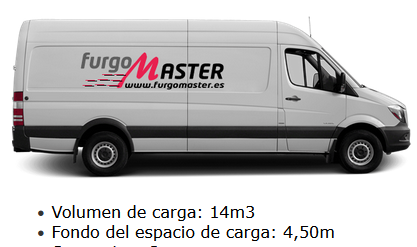
\includegraphics[scale=0.50]{imaxes/FurgonetaBase.png}
  \caption{\label{fig:FurgonetaBase}Ejemplo de la furgoneta base}
\end{figure}

\begin{figure}[H]
  \centering
  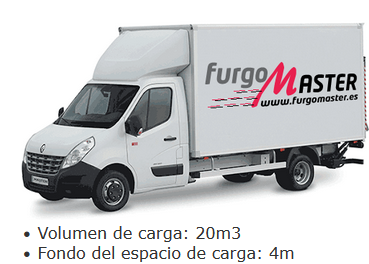
\includegraphics[scale=0.50]{imaxes/FurgonetaFrio.png}
  \caption{\label{fig:FurgonetaFrio}Ejemplo de la furgoneta para cargas en frio}
\end{figure}

\begin{figure}[H]
  \centering
  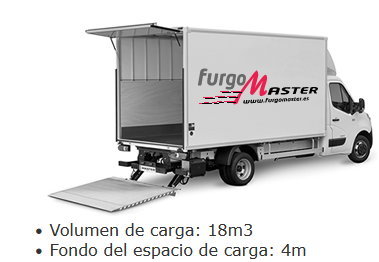
\includegraphics[scale=0.50]{imaxes/FurgonetaAnimales.png}
  \caption{\label{fig:FurgonetaAnimales}Ejemplo de la furgoneta para transportar animales}
\end{figure}

\begin{table}[H]
  \centering
  \resizebox{15,0cm}{!}{
    \begin{tabular}{|c|c|c|c|}
      \hline
      \multicolumn{4}{|c|}{\textbf{Lista de paquetes para asignar recursos para la Ruta A}} \\
      \hline \hline
      
      \multicolumn{1}{|p{1.0cm}|}{\centering \textsc{N\textordmasculine}} &\multicolumn{1}{|p{3.0cm}|}{\centering \textsc{Dimensión (cm)}} & \multicolumn{1}{|p{3.0cm}|}{\centering \textsc{Peso (kg)}} & \multicolumn{1}{|p{3.0cm}|}{\centering \textsc{Tipo de paquete}} \\
      \hline

      1 & \multicolumn{1}{|p{3.0cm}|}{\centering 30x30x30} & \multicolumn{1}{|p{3.0cm}|}{\centering 10} & \multicolumn{1}{|p{3.0cm}|}{\centering normal} \\
      \hline
      2 & \multicolumn{1}{|p{3.0cm}|}{\centering 200x100x40} & \multicolumn{1}{|p{3.0cm}|}{\centering 30} & \multicolumn{1}{|p{3.0cm}|}{\centering normal} \\
      \hline
      3 & \multicolumn{1}{|p{3.0cm}|}{\centering 100x50x40} & \multicolumn{1}{|p{3.0cm}|}{\centering 15} & \multicolumn{1}{|p{3.0cm}|}{\centering frio} \\
      \hline
    \end{tabular}
  }
	\caption{\label{tab:AsignarRecursoRutaA}Lista de paquetes asignados a la Ruta A}
\end{table}

\begin{table}[H]
  \centering
  \resizebox{15,0cm}{!}{
    \begin{tabular}{|c|c|c|c|}
      \hline
      \multicolumn{4}{|c|}{\textbf{Lista de paquetes para asignar recursos para la Ruta B}} \\
      \hline \hline
      
      \multicolumn{1}{|p{1.0cm}|}{\centering \textsc{N\textordmasculine}} &\multicolumn{1}{|p{3.0cm}|}{\centering \textsc{Dimensión (cm)}} & \multicolumn{1}{|p{3.0cm}|}{\centering \textsc{Peso (kg)}} & \multicolumn{1}{|p{3.0cm}|}{\centering \textsc{Tipo de paquete}} \\
      \hline

      1 & \multicolumn{1}{|p{3.0cm}|}{\centering 130x130x130} & \multicolumn{1}{|p{3.0cm}|}{\centering 10} & \multicolumn{1}{|p{3.0cm}|}{\centering normal} \\
      \hline
      
      2 & \multicolumn{1}{|p{3.0cm}|}{\centering 200x200x200} & \multicolumn{1}{|p{3.0cm}|}{\centering 20} & \multicolumn{1}{|p{3.0cm}|}{\centering animal} \\
      \hline
      
      3 & \multicolumn{1}{|p{3.0cm}|}{\centering 100x50x40} & \multicolumn{1}{|p{3.0cm}|}{\centering 15} & \multicolumn{1}{|p{3.0cm}|}{\centering frio} \\
      \hline
    \end{tabular}
  }
	\caption{\label{tab:AsignarRecursoRutaB}Lista de paquetes asignados a la Ruta B}
\end{table}

\begin{table}[H]
  \centering
  \resizebox{15,0cm}{!}{
    \begin{tabular}{|c|c|c|c|}
      \hline
      \multicolumn{4}{|c|}{\textbf{Lista de paquetes para asignar recursos para la Ruta C}} \\
      \hline \hline
      
      \multicolumn{1}{|p{1.0cm}|}{\centering \textsc{N\textordmasculine}} &\multicolumn{1}{|p{3.0cm}|}{\centering \textsc{Dimensión (cm)}} & \multicolumn{1}{|p{3.0cm}|}{\centering \textsc{Peso (kg)}} & \multicolumn{1}{|p{3.0cm}|}{\centering \textsc{Tipo de paquete}} \\
      \hline

      1 & \multicolumn{1}{|p{3.0cm}|}{\centering 130x130x130} & \multicolumn{1}{|p{3.0cm}|}{\centering 10} & \multicolumn{1}{|p{3.0cm}|}{\centering normal} \\
      \hline
      
      2 & \multicolumn{1}{|p{3.0cm}|}{\centering 200x200x200} & \multicolumn{1}{|p{3.0cm}|}{\centering 20} & \multicolumn{1}{|p{3.0cm}|}{\centering animal} \\
      \hline
      
      3 & \multicolumn{1}{|p{3.0cm}|}{\centering 100x50x40} & \multicolumn{1}{|p{3.0cm}|}{\centering 15} & \multicolumn{1}{|p{3.0cm}|}{\centering frio} \\
      \hline
    \end{tabular}
  }
	\caption{\label{tab:AsignarRecursoRutaC}Lista de paquetes asignados a la Ruta C}
\end{table}

Asignar recursos para las siguientes encenarios:
\begin{enumerate}
	\item  \textbf{Listado de carga para la Ruta A:} Asignar recursos para la entrega de la paquetería del listado de la Tabla \ref{tab:AsignarRecursoRutaA}.
	\item  \textbf{Listado de carga para la Ruta B:} Asignar recursos para la entrega de la paquetería del listado de la Tabla \ref{tab:AsignarRecursoRutaB}.
\end{enumerate}

\section{Fase de especificación}
\subsection{Justificación de la selección de la metodología}
Para este proyecto hemos decidido utilizar la metodología ``middle-out'' con la selección de la plantilla de configuración como se muestra en la Figura \ref{fig:PlantillaConfiguracion}, ya que esa plantilla nos permite buscar una mejor distribución de la carga dentro del vehículo asignado a la ruta. 

\begin{figure}[H]
  \centering
  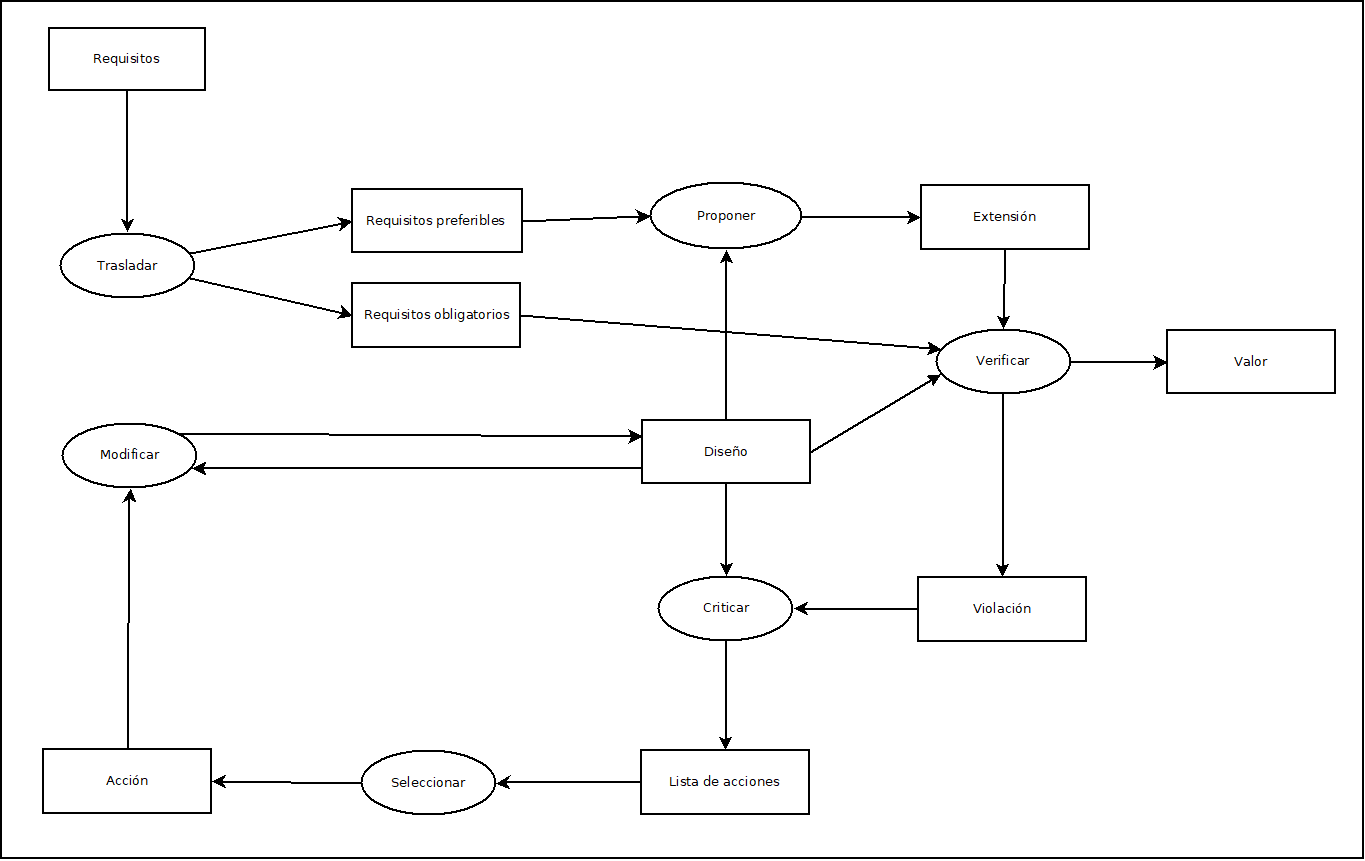
\includegraphics[scale=0.30]{imaxes/PlantillaConfiguracion.png}
  \caption{\label{fig:PlantillaConfiguracion}Ejemplo de la plantilla elegida}
\end{figure}

\subsection{Plantilla anotada}

La plantilla que mas se adapta a nuestro problema es la de configuración, como se muestra en la Figura \ref{fig:PlantillaConfiguracionComentada}.

\begin{figure}[H]
  \centering
  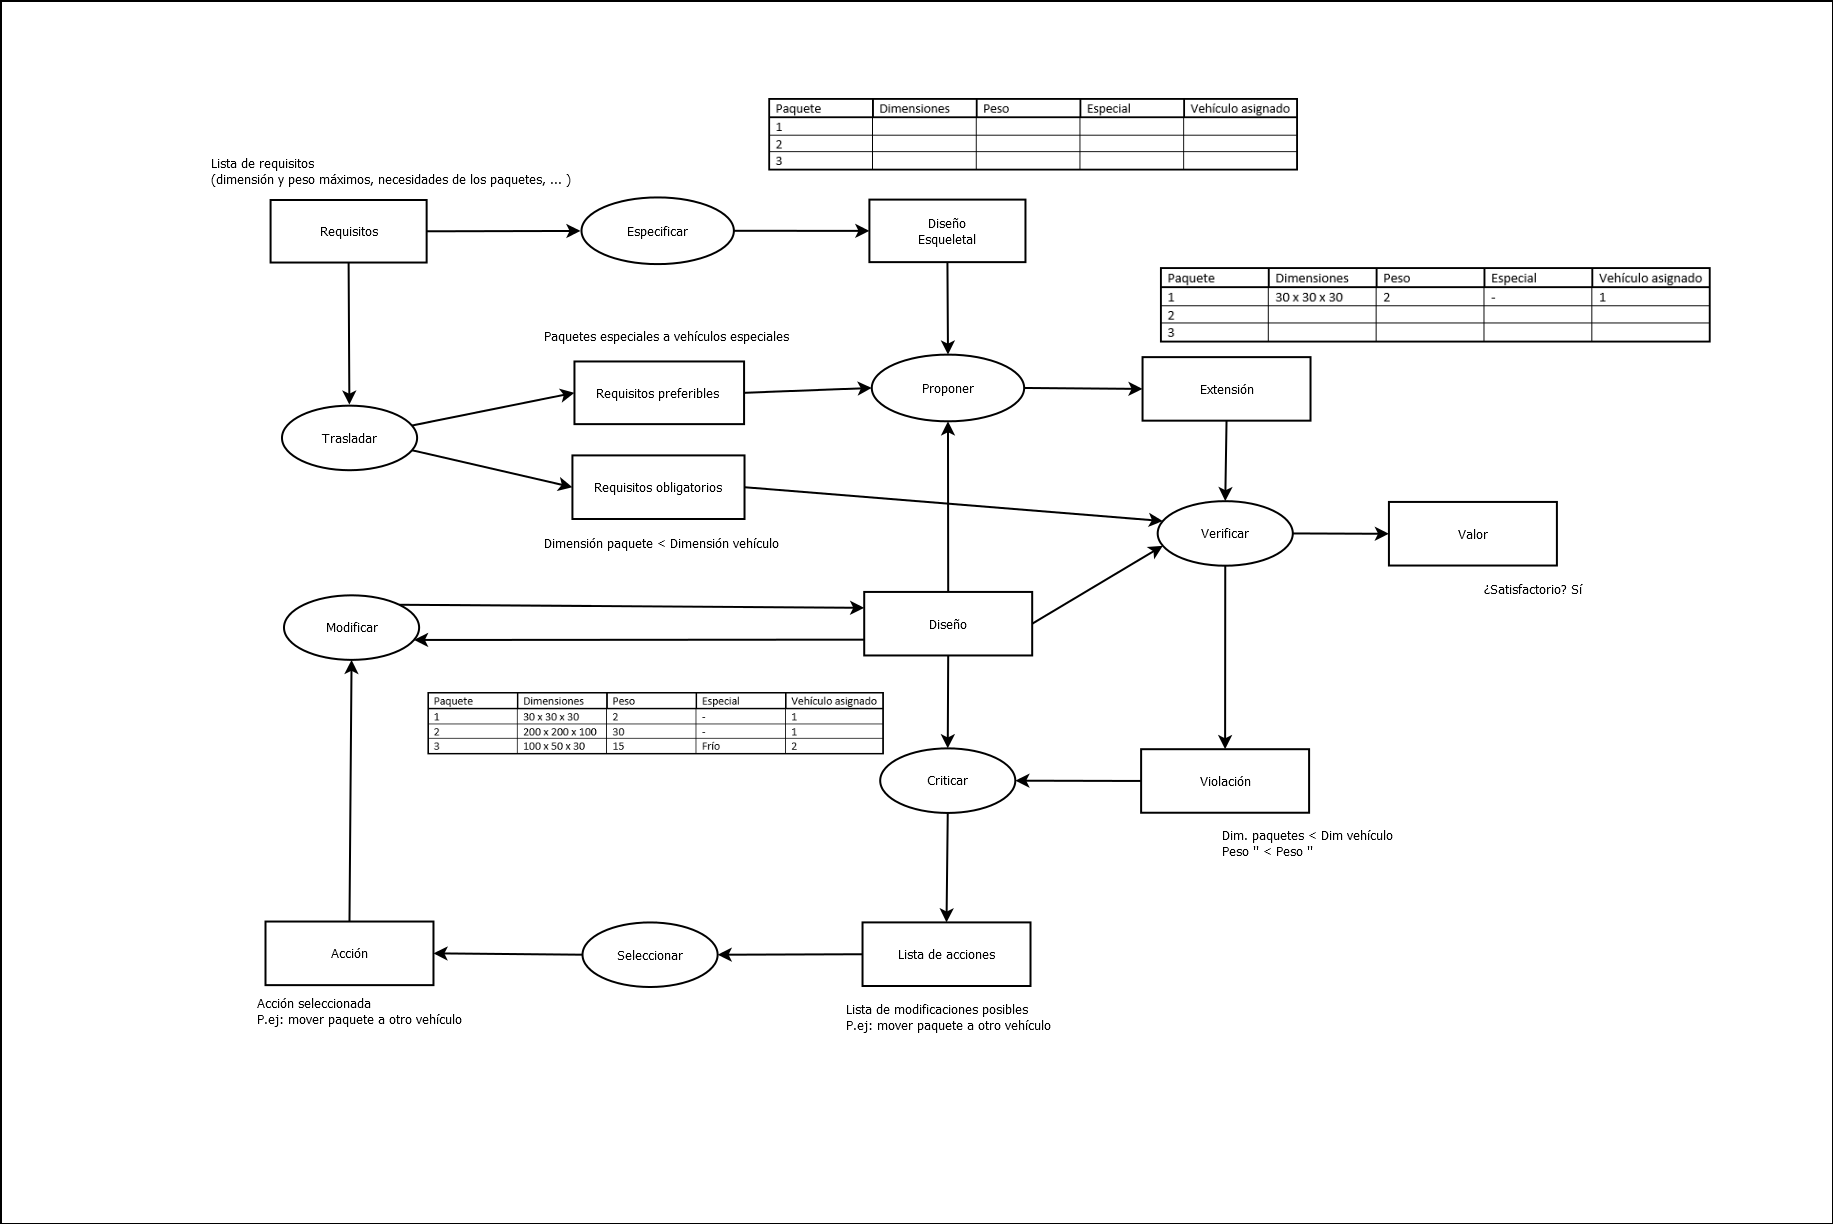
\includegraphics[scale=0.25]{imaxes/PlantillaConfiguracionComentada.png}
  \caption{\label{fig:PlantillaConfiguracionComentada}Ejemplo de la plantilla elegida con las anotaciones pertinentes}
\end{figure}

\newpage

\begin{lstlisting}[language=C,caption=\textbf{Código de la plantilla de configuración}]
  TASK configuracion-diseño;
    ROLES:
      INPUT: Requisitos: "requisitos para el diseño";
      OUTPUT: Diseño: "el diseño resultante";
  END TASK configuracion-diseño;
  TASK-METHOD proponer-y-revisar;
    REALIZES: configuracion-diseño;
    DECOMPOSITION:
      INFERENCES: Trasladar, Especificar, Proponer, Verificar, Criticar, Seleccionar, Modificar;
    ROLES:
      INTERMEDIATE:
        Requisitos-preferibles: "requisitos que se utilizarán como preferencias (suaves)";
        Requisitos-obligatorios: "requisitos que son restricciones obligatorias (estrictas)";
        Diseño-Esqueletal: "conjunto de elementos de diseño";
        Extensión: "un único valor nuevo para un elemento de diseño";
        Violación: "restricción violada por el diseño actual";
        Valor: "booleano que indica el resultado de la verificación";
        Lista-de-acciones: "lista ordenada de posibles acciones de reparación (fijación)";
        Acción: "una sola acción de reparación";
    CONTROL-STRUCTURE:
      operationalize(Requisitos -> Requisitos-deseables + Requisitos-necesarios);
      specify(Requisitos -> Diseño-Esqueletal);
      WHILE NEW-SOLUTION propose(Diseño-Esqueletal + Diseño + Requisitos-necesarios -> Extensión) DO
        Diseño := Extension ADD Diseño;
        verify(Diseño + Requisitos-deseables -> Valor + Violación);
        IF Valor == false
        THEN
          critique(Violación + Diseño -> Lista-de-acciones);
          REPEAT
            select(Lista-de-acciones -> Acción);
            modify(Diseño + Acción -> Diseño);
            verify(Diseño + Requisitos-deseables -> Valor + Violación);
          UNTIL Valor == true;
          END REPEAT
        END IF
      END WHILE
  END TASK-METHOD proponer-y-revisar;
\end{lstlisting}

\subsection{Esquema inicial del dominio}
La Figura \ref{fig:DiagramaInicialDominio} muestra el diagrama inicial del dominio.
\begin{figure}[H]
  \centering
  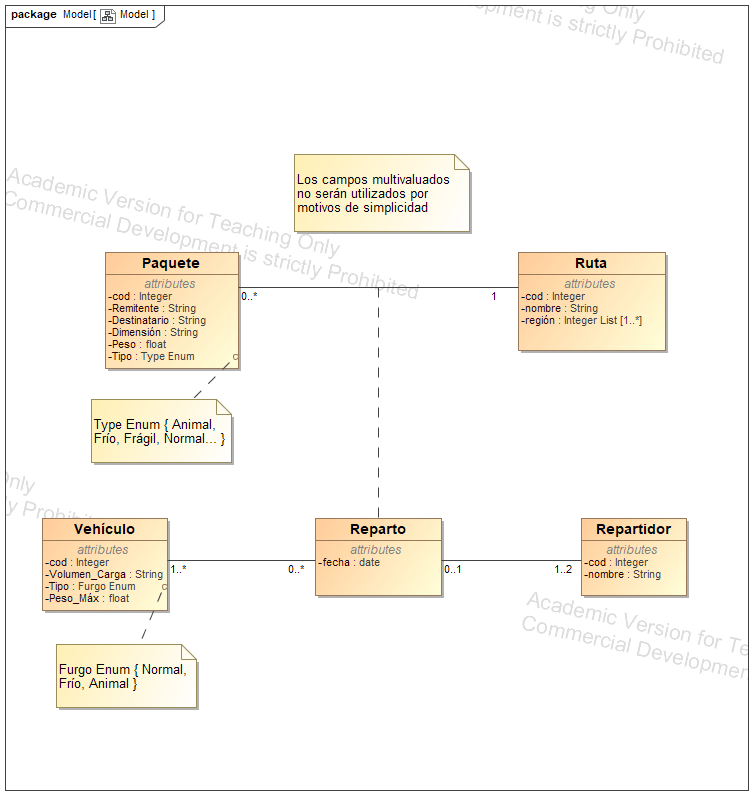
\includegraphics[scale=0.50]{imaxes/DiagramaInicialDominio.png}
  \caption{\label{fig:DiagramaInicialDominio}Diagrama inicial del dominio}
\end{figure}

\subsection{Estructura inferencial}

La Figura \ref{fig:EstructuraInferencial} muestra la estructura inferencial de la plantilla elegida.
\begin{figure}[H]
  \centering
  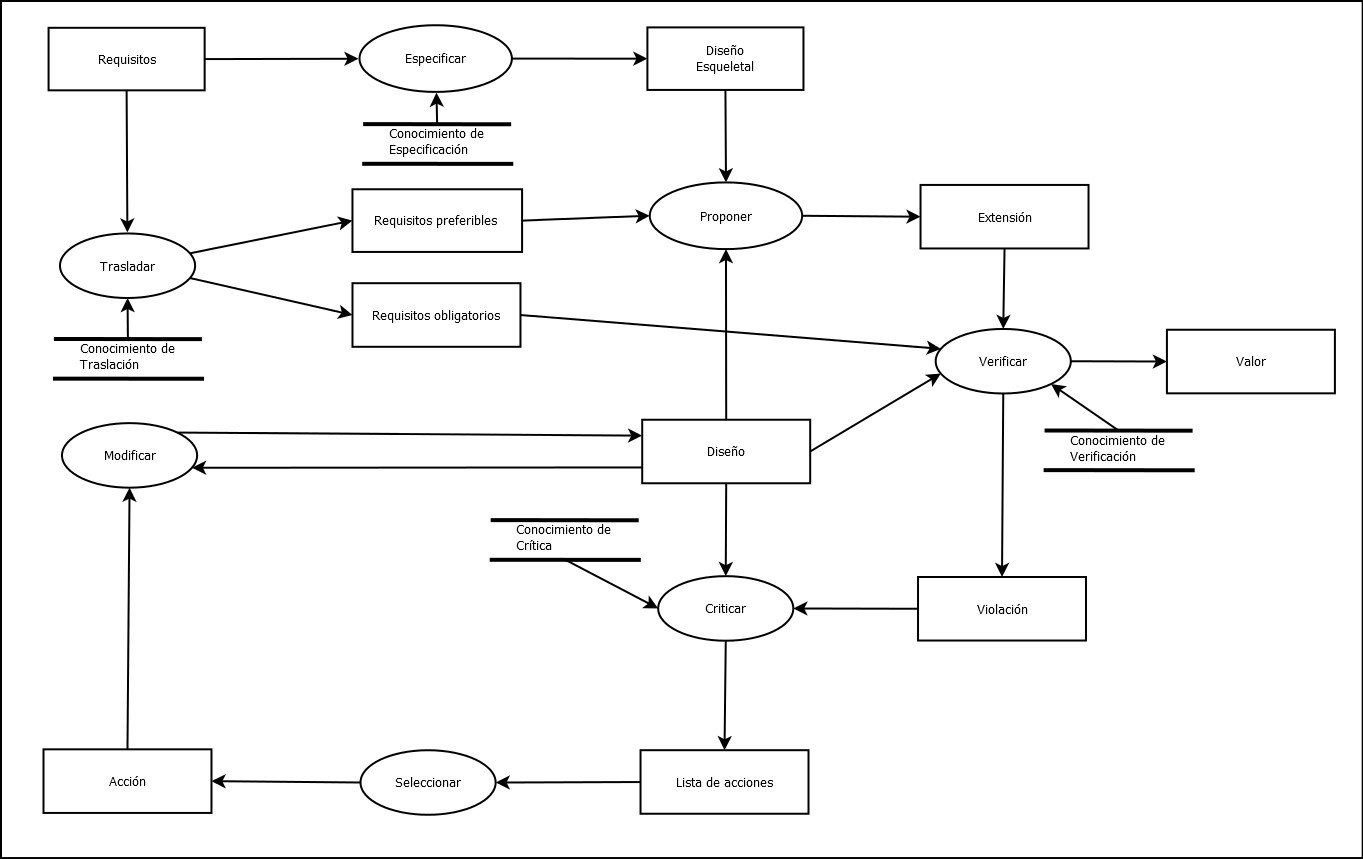
\includegraphics[scale=0.50]{imaxes/EstructuraInferencial.png}
  \caption{\label{fig:EstructuraInferencial}Estructura inferencial de la plantilla elegida}
\end{figure}